%% SpatialNet -- IMWUT submission.
%% Build: pdflatex main && bibtex main && pdflatex main && pdflatex main   (see README.md)
%% Red text marks the real-frame check (T5), still to be filled in.
\documentclass[acmsmall,screen,review,anonymous]{acmart}
\acmJournal{IMWUT}

\usepackage{multirow}
\usepackage{rotating}

%% ---- Draft markers (only the T5 real-frame check uses them; delete with it) ----
\newcommand{\tbd}[1]{\textcolor{red}{[#1]}}                 % text to write or confirm
\newcommand{\xx}{\textcolor{red}{xx.x}}                      % numeric result to fill in
\newcommand{\phfig}[3]{\fcolorbox{red}{white}{\parbox[c][#2][c]{\dimexpr#1-2\fboxsep-2\fboxrule\relax}{\centering\color{red}\footnotesize #3}}}

\newlength{\archh}   % height of the sideways architecture figure (set before the float)

%% ---- Notation ----
\newcommand{\vect}[1]{\mathbf{#1}}
\newcommand{\bH}{\vect{b}_h}
\newcommand{\bT}{\vect{b}_t}
\newcommand{\cH}{\vect{c}_h}
\newcommand{\cT}{\vect{c}_t}
\newcommand{\vH}{\vect{v}_h}
\newcommand{\vP}{\vect{v}_p}
\newcommand{\tip}{\vect{p}}
\newcommand{\dir}{\vect{u}}
\newcommand{\cell}{\vect{g}}

\begin{document}

\title[SpatialNet]{SpatialNet: Compact Pointing-Target Localisation
for Smart Glasses with Wearer-Aware Hand Ownership}

\author{Anonymous Author(s)}
\affiliation{%
  \institution{Anonymous Institution}
  \country{Anonymous Country}}

\begin{abstract}
Pointing is the most direct way to ask smart glasses about something in view (``what is \emph{that}?''). Before any assistant can answer, the glasses must work out which object the wearer is pointing at, from their own camera and quickly. Current pointing-grounding models are transformers and multimodal LLMs with hundreds of millions to billions of parameters. They run on GPUs, the LLMs decode their answers token by token, and some models need a text prompt or the hand box as input. We ask how far a model that fits on the glasses can go.

SpatialNet takes nothing but one 2D RGB frame: no text, no hand box, no depth, no external hand or pose model. In a single forward pass of a compact convolutional network without self-attention (0.72M parameters, 0.23 GFLOPs, 1.6\,MB in FP16), it outputs the wearer's hand, the fingertip, the pointing direction and the box of the pointed-at object. To make this possible at that size, its heads form an instance-anchored chain: each stage reads a shared feature map where the previous stage predicted, so the hand, fingertip, direction and target stay on one hand.

On the EgoPoint test split, SpatialNet finds the wearer's hand with a P@0.5 of 92.6\% (share of frames with IoU $\geq$ 0.5) and localises the pointed-at object with a P@0.5 of 58.9\% (mIoU 53.3\%; 58.9--59.0\% across three training seeds). This is comparable to zero-shot 7--8B multimodal LLMs reported on the same split (44.5--49.8\% P@0.5) and below models of 226M--7B parameters trained on EgoPoint (63.6--93.9\%). It drops to 25.4\% for objects far from the fingertip. Compact detectors that we trained on the same data at the same compute (YOLO26n, NanoDet-Plus-m; 1.6--3.5 times the parameters) draw tighter boxes and reach 59.9--67.6\% P@0.5. SpatialNet places the box centre on the right object slightly more often (84.8\% against 81.6--82.9\%), and it is the only model whose accuracy does not drop when other hands are pasted into view. Ablations and a resolution study show what matters at this scale:
\begin{itemize}
\item the anchoring keeps the hand box and direction precise (without it, hand mIoU drops by 1.8 points and the direction error rises by 3.4$^\circ$);
\item input resolution is the largest lever (65.1\% at 320\,px with the same parameters);
\item a learned prior from explicit ray geometry, which we also test, collapses into a fingertip-proximity prior on EgoPoint's touch-dominated data.
\end{itemize}
On an engineering unit of a pair of smart glasses, the 160\,px model runs in 60--80\,ms per frame, and running it continuously drains less battery than merely streaming frames to a phone.
\end{abstract}

\ccsdesc[500]{Human-centered computing~Ubiquitous and mobile computing systems and tools}
\ccsdesc[500]{Human-centered computing~Gestural input}
\ccsdesc[300]{Computing methodologies~Object detection}

\keywords{smart glasses, pointing gesture, deictic reference, egocentric vision, on-device inference, efficient neural networks}

\begin{teaserfigure}
  \centering
  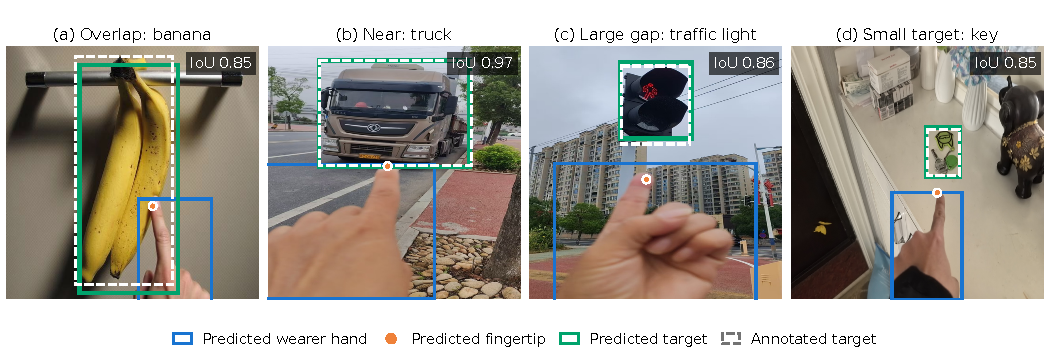
\includegraphics[width=\textwidth]{figures/teaser_successes}
  \caption{SpatialNet's predictions from a single frame: the wearer's hand (blue), the fingertip (orange) and the pointed-at object (green); white dashed: labelled object. The examples cover a touched target (a), a near target (b), a far target (c) and a small, far target (d). Boxes, points and IoUs are the saved predictions of the 160\,px model on EgoPoint test images. These are deliberately selected successes, not average accuracy; complex failures are shown in Figure~\ref{fig:failures}.}
  \Description{Four egocentric photos with predicted boxes that match the labelled boxes: a banana touched by the finger (IoU 0.85), a truck near the fingertip (IoU 0.97), a traffic light far from the fingertip (IoU 0.86), and a small key on a wall (IoU 0.85).}
  \label{fig:teaser}
\end{teaserfigure}

\maketitle

\section{Introduction}\label{sec:intro}

Camera-equipped smart glasses are becoming everyday devices, and an assistant on them is most useful when the wearer can refer to things in view. Pointing is the most direct way to do so: ``what is \emph{that}?'', ``remind me to buy \emph{this}''. Systems have combined speech with pointing since Bolt's \emph{Put-that-there}~\cite{bolt1980put}, and recent wearable assistants use pointing and gaze to resolve such pronouns~\cite{lee2024gazepointar}. Before any of this works on glasses, the device must answer a spatial question from its own camera: \emph{which object is the wearer pointing at?}

Answering this on glasses is hard for three reasons.
\begin{itemize}
\item \emph{The egocentric view.} The camera sees the wearer's hand from behind and often only in part. The target may be touched or across the room, and a pointing direction drawn in the image is only a rough guide to it.
\item \emph{Other people's hands.} A companion's hand or a stranger's pointing gesture can be in view, and must not be mistaken for the wearer's.
\item \emph{The budget.} Glasses-class processors share a battery of a few hundred milliampere-hours with the camera, audio and radio. Sending frames to a cloud model adds network latency and moves imagery of bystanders off the device.
\end{itemize}

\paragraph{Prior work.} Pointing-target grounding in egocentric images is an active research area, and EgoPoint-Ground~\cite{egopoint} provides a large benchmark for it. The strongest methods are large models:
\begin{itemize}
\item multimodal LLMs that reason step by step from the hand to a ray and then to the target~\cite{egopoint,li2026pointvgr};
\item a 226M-parameter transformer that models the pointing ray explicitly~\cite{li2026vistaref}.
\end{itemize}
Some benchmark tasks even give the model the ground-truth hand box~\cite{egopoint}. These systems reach high accuracy on a GPU, but none of them is designed for glasses-class hardware, and to our knowledge none addresses other people's hands in view. Egocentric fingertip systems, including one that runs on a phone, stop at the fingertip~\cite{huang2016pointing,jain2019gestarlite} and never localise the target.

\paragraph{SpatialNet.} We ask how far a model that fits on the glasses can go. SpatialNet needs only one 2D RGB frame:
\begin{itemize}
\item no text prompt, no hand box, no depth;
\item no external hand detector or pose estimator.
\end{itemize}
It predicts the wearer's hand, the fingertip, the pointing direction and the box of the pointed-at object, with presence gates for each. All outputs come from one forward pass of a compact convolutional network with no self-attention and no token-by-token decoding: 0.72M parameters, 0.23 GFLOPs, 1.6\,MB in FP16. This makes it 300 times smaller than VistaRef and about 10{,}000 times smaller than the 7B multimodal LLMs.

One design choice lets such a small network localise precisely: \emph{instance-anchored heads}. The heads form a chain in which each one reads a shared feature map at the location the previous one predicted, so the fingertip, direction and target all belong to the same hand.

We also give the target head the geometry of the predicted ray, as six ray-coordinate maps entering through a zero-initialised branch. We then test whether a model this small makes use of it, rather than assuming so. Training additionally pastes unlabelled hands of other people into the frames and penalises responses to them, so the model learns to prefer the wearer's hand without labelled bystander hands.

\paragraph{Evaluation.} We train and test on EgoPoint and report:
\begin{itemize}
\item accuracy by fingertip--target distance, which matters because about 70\% of targets are touched by the fingertip;
\item comparisons with published results of state-of-the-art models and zero-shot multimodal LLMs on the same test split, and with simple fingertip-based references;
\item comparisons with compact detectors (YOLO26n and NanoDet-Plus-m) that we trained on the same split, at the same compute, and scored with the same code;
\item ablations of each component;
\item behaviour when other people's hands are in view (pasted and real);
\item latency, memory and battery drain on an engineering unit of a pair of smart glasses.
\end{itemize}
\paragraph{Results in brief.}
\begin{itemize}
\item SpatialNet finds the wearer's hand reliably (P@0.5 of 92.6\%, the share of test frames with IoU${\geq}0.5$) and the fingertip precisely (3.9\,px mean error at $160\times160$).
\item It localises the pointed-at object with a P@0.5 of 58.9\% (mIoU 53.3\%). That is comparable to zero-shot 7--8B multimodal LLMs reported on the same test split (44.5--49.8\%), close to a 7B model fine-tuned on EgoPoint (63.6\%), and far below VistaRef (93.9\%) and PointVG-R (83.6\%).
\item At the same compute, compact detectors with 1.6--3.5 times the parameters draw tighter boxes (P@0.5 59.9--67.6\%), but SpatialNet places the target centre on the right object at least as often (84.8\% against 81.6--82.9\%), and only SpatialNet keeps its accuracy when other hands are pasted into view.
\item It drops to 25.4\% for far targets. Trained at higher input resolution, with no new parameters, the same model reaches 62.4\% at 224\,px (far: 35.9\%) and 65.1\% at 320\,px (Section~\ref{sec:resolution}).
\item It runs in 60--80\,ms per frame on the glasses. Running it continuously costs less battery (9\% per minute on the test unit) than streaming frames to a phone at 0.5\,fps (16\%).
\end{itemize}
We present this as an operating point, with its limits measured, not as a replacement for large models.

\paragraph{Contributions.}
\begin{enumerate}
\item \emph{An image-only, single-pass pointed-target localiser that runs on smart glasses.}
  \begin{itemize}
  \item From one RGB frame, a 0.72M-parameter CNN without self-attention, external models or prompts outputs the hand, fingertip, direction and target box.
  \item On a smart-glasses engineering unit it takes 60--80\,ms per frame, and running it continuously costs less battery than streaming frames off the device (Sections~\ref{sec:method}, \ref{sec:device} and~\ref{sec:ondevice}).
  \end{itemize}
\item \emph{Instance-anchored heads that keep a sub-million-parameter model precise.} Against a plain model of the same size, the anchoring improves:
  \begin{itemize}
  \item the hand box, by 1.8 points of mIoU;
  \item the direction, by 3.4$^\circ$;
  \item P@0.7, by 2.8 points (1.7 on the test split without duplicates, where the interval reaches zero);
  \item small targets, by 11.3 points.
  \end{itemize}
  The first two gains are well beyond the variation between training seeds; the last two are supporting evidence (Sections~\ref{sec:heads} and~\ref{sec:ablations}).
\item \emph{An analysis of what limits pointing localisation at this scale.}
  \begin{itemize}
  \item Input resolution is the largest lever, at no parameter cost.
  \item Distractor pasting makes the model robust to other hands at no cost on clean images.
  \item A prior learned from explicit ray geometry collapses into a fingertip-proximity prior when most targets are touched. This explains why far targets stay hard, and indicates how future models should constrain the ray (Sections~\ref{sec:resolution}--\ref{sec:own}).
  \end{itemize}
\item \emph{An evaluation that places accuracy next to cost.} It compares with published models that are 300 to 10{,}000 times larger and with compact detectors re-trained at the same compute, stratifies by fingertip--target distance, and decomposes the errors (Section~\ref{sec:results}).
\end{enumerate}
Distractor pasting is treated as a supporting result rather than a headline contribution. Its effect is clear (Section~\ref{sec:ablations}), but its test distractors are synthetic.

\section{Related Work}\label{sec:related}

\paragraph{Pointing as input.} Deictic gestures have been part of multimodal interfaces since \emph{Put-that-there}~\cite{bolt1980put}. Studies of mid-air pointing show that both the hand and the eye matter. Ray-casting models of pointing have systematic offsets~\cite{mayer2015modeling}, and taking the dominant eye and handedness into account makes them markedly more accurate~\cite{plaumann2018towards}. On wearables, GazePointAR combines gaze, pointing and conversation history to resolve spoken pronouns in AR~\cite{lee2024gazepointar}. EgoPointVQA asks questions about pointed-at objects in egocentric video and feeds 3D hand keypoints, estimated by an off-the-shelf model, to a multimodal LLM as hand-intent tokens~\cite{choi2026hint}. These systems show the value of pointing on wearables; SpatialNet supplies the localisation step that such systems need, at a cost that fits on the glasses.

\paragraph{Fingertips and pointing directions.} EgoFinger detects the hand and fingertip in egocentric video for air-writing~\cite{huang2016pointing}. GestARLite runs a hand detector, a fingertip regressor and a gesture classifier on a smartphone~\cite{jain2019gestarlite}. DeePoint recognises pointing and estimates its 3D direction from third-person video of the whole body~\cite{nakamura2023deepoint}. None of these localises the object being pointed at.

\paragraph{Pointing-target grounding.}
\begin{itemize}
\item \emph{Third-person.} YouRefIt grounds targets from language and gesture together~\cite{chen2021yourefit}.
\item \emph{EgoPoint-Ground.} For egocentric images, it introduced 15K images (real captures from smart glasses, plus synthetically composed and generated images) and several tasks~\cite{egopoint}. In its pointing-only task, models receive the image and the ground-truth hand box and are evaluated without task-specific training. Its SV-CoT baseline reasons with a multimodal LLM from the pointing direction to a ray and then to the target.
\item \emph{PointVG-R.} It builds a similar hand--direction--ray--target chain of thought into Qwen2.5-VL-7B with reinforcement learning~\cite{li2026pointvgr}, and names latency as a limitation for wearables.
\item \emph{VistaRef.} It adds hand-keypoint and geometric-ray modules and an orientation-consistency loss to a BEiT-3 grounding model (226M parameters with the Base backbone)~\cite{li2026vistaref}. With the Large backbone, it reports a P@0.5 of 93.9\% (mIoU 82.0\%) on the 3,072 EgoPoint test images (Section~\ref{sec:data} explains how our test split differs).
\item \emph{EgoPoint-Bench.} It shows that general multimodal LLMs still struggle with egocentric pointing~\cite{li2026egopointbench}.
\end{itemize}
Explicit ray reasoning is thus not new, and neither is avoiding a hand-box input: VistaRef uses a fixed prompt and finds the hand itself. What SpatialNet changes is the operating point:
\begin{itemize}
\item the only input is the image;
\item it uses no language model, no transformer and no external pose model;
\item a single forward pass of a 0.72M-parameter CNN, 300--10{,}000 times smaller than the models above, produces every output;
\item we test, rather than assume, whether explicit ray geometry helps a model this small, and show when it does not;
\item it runs on smart-glasses hardware.
\end{itemize}
Table~\ref{tab:related} summarises the differences.

\paragraph{Hands of the wearer and of others.} Egocentric hand datasets have long distinguished the camera wearer's hands from other people's: EgoHands labels \emph{my} and \emph{your} left and right hands~\cite{bambach2015lending}. Large-scale hand detectors model hand side and contact state~\cite{shan2020understanding}. Pointing datasets, EgoPoint included, contain only the wearer's hand. We therefore synthesise other people's hands with copy-paste augmentation~\cite{dwibedi2017cut,ghiasi2021simple}. Unlike in standard copy-paste, the pasted instances are deliberately left unlabelled and penalised.

\paragraph{Efficient localisation and grounding.} Our trunk follows efficient detection design~\cite{ma2018shufflenet,tan2020efficientdet}. Our heads predict keypoint heatmaps in the manner of CenterNet~\cite{zhou2019objects}, with a differentiable soft-argmax~\cite{sun2018integral}. Open-vocabulary detectors and multimodal LLMs can ground text queries~\cite{liu2024grounding,peng2023kosmos,you2024ferret,bai2025qwen25vl}, but pointing is not text, and their size rules them out for continuous use on glasses.

\begin{table}[t]
  \caption{Methods that localise pointing or its target. \emph{Hand box}: the ground-truth hand box is an input. Parameter counts as reported; ``$>$1B'': built on a multimodal LLM.}
  \label{tab:related}
  \footnotesize
  \setlength{\tabcolsep}{3pt}
  \begin{tabular}{lllllll}
    \toprule
    Method & View & Test-time input & Output & Params & On device & Other hands \\
    \midrule
    EgoFinger~\cite{huang2016pointing} & ego & image & fingertip & -- & -- & -- \\
    GestARLite~\cite{jain2019gestarlite} & ego & frames & fingertip, gesture & 16.3\,MB & phone & -- \\
    DeePoint~\cite{nakamura2023deepoint} & 3rd & video & pointing, 3D direction & -- & -- & -- \\
    YouRefIt~\cite{chen2021yourefit} & 3rd & image + language & target box & -- & -- & -- \\
    SV-CoT (POG)~\cite{egopoint} & ego & image + hand box & target box & $>$1B & -- & -- \\
    PointVG-R~\cite{li2026pointvgr} & ego & image + instruction & target box & 7B & -- & -- \\
    VistaRef~\cite{li2026vistaref} & ego & image + fixed prompt & target box, keypoints & $\geq$226M & -- & -- \\
    \textbf{SpatialNet} & ego & image & hand, tip, ray, target & 0.72M & glasses & trained \\
    \bottomrule
  \end{tabular}
\end{table}

\section{Problem Definition}\label{sec:problem}

\paragraph{Outputs.} Given one RGB frame from a head-worn camera, SpatialNet predicts:
\begin{enumerate}
\item three presence flags $(H,P,T)$: the wearer's hand is visible, the hand is pointing, and something is pointed at;
\item the box $\bH$ of the wearer's hand;
\item the fingertip $\tip$;
\item the pointing direction $\dir$ in the image plane;
\item the box $\bT$ of the pointed-at object, which we call the \emph{target}.
\end{enumerate}
Boxes are $(c_x,c_y,w,h)$ and points $(x,y)$, both normalised to $[0,1]$. The flags combine into four scenes that an interface can act on: 000 \emph{no hand}, 100 \emph{hand, not pointing}, 110 \emph{pointing, no target} and 111 \emph{pointing at a target}.

\paragraph{What separates this from generic detection.}
\begin{itemize}
\item \emph{Ownership.} When several hands are visible, $\bH$, $\tip$ and $\bT$ must refer to the wearer's hand, and a frame showing only other people's hands is \emph{no hand}.
\item \emph{Budget.} The model must run on the glasses' own processor, within an interactive latency, without a second network or a server call.
\end{itemize}

\paragraph{Scope.} We do not recognise \emph{what} the target is. $\bT$ is the region that a later step would take as input: an object recogniser, a visual question-answering model or an application. Localising the region first means that this step can run on a small crop instead of the full frame, and only when a pointing event occurs. The cost of that later step is outside the scope of this paper.

\section{SpatialNet}\label{sec:method}

Figure~\ref{fig:arch} shows the complete network. A shared trunk turns the frame into one feature map. Four heads then run in a fixed order (wearer's hand, fingertip, pointing direction, pointed target), and each head reads the shared map \emph{at the location that the previous head predicted}. We call these heads \emph{instance-anchored}: the fingertip is searched for around the hand that was found, the direction is computed from features of that hand and fingertip, and the target is searched for along the resulting ray. Three small gates decide which outputs are valid. Everything is a single forward pass; there is no external hand detector, no language input, and no hand box at test time.

\begin{figure}[t]
  \centering
  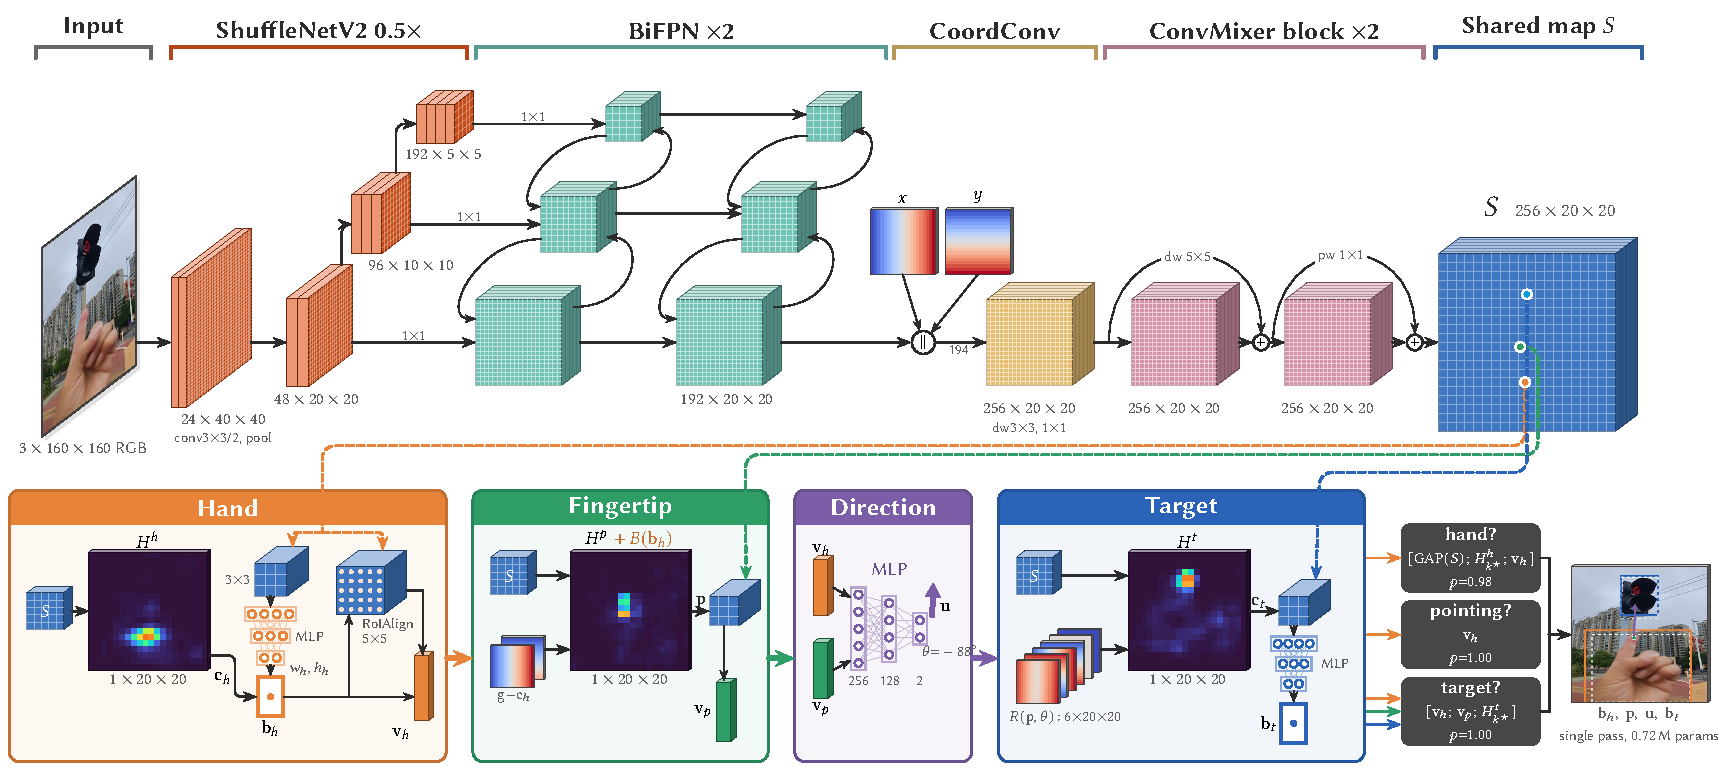
\includegraphics[width=\textwidth]{figures/architecture}
  \caption{SpatialNet. The trunk (top) turns one $160\times160$ frame into the shared map $S$ ($256\times20\times20$): ShuffleNetV2 stages at strides 8, 16 and 32, two BiFPN layers, CoordConv with reduction to 256 channels, and two ConvMixer blocks. Four heads (middle) run in order. Dashed lines mark where a head samples $S$ at the location the previous head predicted: the hand centre $\cH$, the fingertip $\tip$ and the target centre $\cT$. The direction head reads only the descriptors $\vH,\vP$. Right: the presence gates and the decoded output. Heatmaps, offset and ray-coordinate maps, gate probabilities and the output are real outputs of the trained model on one test image.}
  \Description{Block diagram drawn as three-dimensional tensor slabs. The input frame passes through a ShuffleNetV2 backbone whose three scales feed two BiFPN layers by 1x1 projections; the 20x20 output gets two coordinate channels, is reduced to 256 channels and passes two ConvMixer blocks to give the shared map S. Four coloured panels show the heads in sequence: wearer hand (heatmap, 3x3 sample and MLP for the box size, RoIAlign descriptor), fingertip (heatmap from S and offset channels to the hand centre plus a hand-box prior, 3x3 sample giving the fingertip descriptor), pointing direction (an MLP on the hand and fingertip descriptors giving a unit vector), and pointed target (six ray-coordinate maps and S giving the target heatmap, 3x3 sample and MLP giving the box). Dashed lines from S show where each head samples it. On the right, three presence gates list their inputs and probabilities, and the output frame shows the predicted hand box, fingertip, direction and target box.}
  \label{fig:arch}
\end{figure}

\subsection{Shared Trunk}\label{sec:trunk}
The frame is resized to $160\times160$. A ShuffleNetV2~0.5$\times$ backbone~\cite{ma2018shufflenet} (stages 2--4 only; ImageNet-pretrained~\cite{deng2009imagenet}) gives feature maps at strides 8, 16 and 32. Two BiFPN layers~\cite{tan2020efficientdet} merge them into one $192\times20\times20$ map at stride 8. Each fused map is smoothed by a depthwise $3\times3$ convolution, SiLU, and parameter-free SimAM attention~\cite{yang2021simam}. We then append two coordinate channels (CoordConv~\cite{liu2018coordconv}) and reduce to $D{=}256$ channels with a depthwise-separable convolution. Two ConvMixer-style residual blocks~\cite{trockman2023patches} follow, each made of a depthwise $5\times5$ and a pointwise convolution with residual connections. Their batch-norm scales start at zero, so each block is the identity at initialisation. The output is the shared map $S\in\mathbb{R}^{256\times20\times20}$, which all heads read.

A $20\times20$ grid gives 8-pixel cells at the model input. The heads recover points with sub-cell precision (Section~\ref{sec:softargmax}), so a finer grid would mostly add compute. Sharing one map keeps the heads cheap: the largest head has 104K parameters (Table~\ref{tab:params}).

\subsection{Locating One Instance: Peak-Windowed Soft-Argmax}\label{sec:softargmax}
Each head predicts a $20\times20$ logit map $H$ and turns it into a point. A global soft-argmax~\cite{sun2018integral} returns the probability-weighted mean over all cells. When two hands are visible, that mean falls \emph{between} them. We therefore restrict the softmax to a $(2r{+}1)\times(2r{+}1)$ window $\mathcal{W}$ around the arg-max cell $k^\star$:
\begin{equation}
\pi_k=\frac{\mathbb{1}[k\in\mathcal{W}]\,\exp(\tau H_k)}{\sum_{j\in\mathcal{W}}\exp(\tau H_j)},\qquad
\hat{\vect{c}}=\sum_k \pi_k\,\cell_k ,
\label{eq:softargmax}
\end{equation}
where $\cell_k\in[0,1]^2$ is the normalised position of cell $k$ and $\tau$ is a temperature. The estimate follows a single peak, is differentiable within the window, and is not limited to cell centres. We use $(\tau,r)=(8,2)$ for the hand and the target and $(10,1)$ for the fingertip. The peak logit $H_{k^\star}$ is also passed to the gates as a confidence cue.

\subsection{Instance-Anchored Heads}\label{sec:heads}

\paragraph{Wearer's hand.} A depthwise $3\times3$ and pointwise head gives hand-centre logits $H^h$, and Eq.~\eqref{eq:softargmax} gives the centre $\cH$. For the box size $(w_h,h_h)$, we sample a $3\times3$ neighbourhood of $S$ around $\cH$ bilinearly (one-cell spacing). A depthwise $3\times3$ convolution and a pointwise projection collapse it to 128 dimensions, and a two-layer MLP with a sigmoid maps it to the size, giving $\bH=(\cH,w_h,h_h)$. To describe \emph{this} hand instance, we sample a $5\times5$ RoIAlign-style lattice~\cite{he2017mask} over $\bH$ enlarged by 1.15. This lattice is collapsed to 128 dimensions and fused with the box coordinates into the hand descriptor $\vH\in\mathbb{R}^{128}$.

\paragraph{Fingertip.} The fingertip must belong to the hand just found. Its logits add three terms:
\begin{equation}
H^p = V^p(S) + G^p\big([S;\,\alpha_p(\cell-\cH)]\big) + B(\bH),
\label{eq:tip}
\end{equation}
\begin{itemize}
\item $V^p$ is a visual head of the same form as the hand head.
\item $\alpha_p(\cell-\cH)$ are two channels holding each cell's offset to the hand centre; $\alpha_p$ is a learnable scale.
\item $G^p$ is a small branch (a $1\times1$ convolution to 48 channels, then a $3\times3$ convolution to one channel) that learns where fingertips lie relative to the hand centre. Its last layer starts at zero.
\item $B$ is a fixed log-prior. It is zero inside the hand box dilated by $\delta{=}1.3$ and falls linearly outside it:
\begin{equation}
B_k(\bH) = -\frac{\lambda}{\tau_p}\Big(\big[\tfrac{|g_{k,x}-c_{h,x}|}{\delta w_h/2}-1\big]_+ + \big[\tfrac{|g_{k,y}-c_{h,y}|}{\delta h_h/2}-1\big]_+\Big),
\end{equation}
where $[\cdot]_+=\max(\cdot,0)$. With $\lambda{=}4$, the penalty after the softmax temperature $\tau_p$ is 4 logits for every half box-width outside the dilated box. No gradient flows from the prior into $\bH$.
\end{itemize}
In the training labels, the fingertip lies inside the dilated box in 99.4\% of pointing images, so the prior rarely contradicts a label, while it rules out the fingertips of other hands. Eq.~\eqref{eq:softargmax} (with $r{=}1$) gives the fingertip $\tip$, and a $3\times3$ sample around it gives the fingertip descriptor $\vP\in\mathbb{R}^{128}$.

\paragraph{Pointing direction.} An MLP ($256\to128\to2$, $\tanh$) maps $[\vH;\vP]$ to a vector. We L2-normalise it into the unit direction $\dir=(\cos\theta,\sin\theta)$ in image coordinates. The direction is supervised with the image-plane direction from the labelled fingertip to the labelled target centre (Section~\ref{sec:losses}). $\dir$ is therefore the direction \emph{to the target} as it appears in the image, not the 3D orientation of the finger.

\paragraph{Pointed target.} The target head is given the geometry of the predicted ray explicitly. From $\tip$ and $\dir$, every cell $k$ receives six \emph{ray coordinates} (inset in Figure~\ref{fig:arch}):
\begin{equation}
\Delta_k=\alpha_t(\cell_k-\tip),\qquad
t_k=\Delta_k\cdot\dir,\qquad
s_k=\big|\Delta_{k,x}\sin\theta-\Delta_{k,y}\cos\theta\big|,\qquad
\cos\theta,\qquad \sin\theta .
\label{eq:raycoords}
\end{equation}
These are:
\begin{itemize}
\item $\Delta_k$ (two channels): the scaled offset from the fingertip;
\item $t_k$: the signed distance along the ray, negative behind the fingertip;
\item $s_k$: the distance from the line of the ray;
\item $\cos\theta$ and $\sin\theta$: the direction itself.
\end{itemize}
The target logits are
\begin{equation}
H^t = V^t(S) + G^t\big([S;\,R(\tip,\theta)]\big),
\label{eq:target}
\end{equation}
where $R$ stacks the six maps, and $G^t$ (13K parameters) has the form of $G^p$ and also starts at zero. The soft-argmax applies a softmax to $\tau H^t$, so $\pi_k\propto\exp(\tau V^t_k)\exp(\tau G^t_k)$: the geometry term acts as a learned \emph{multiplicative prior} on the visual evidence. Because $G^t$ starts at zero, training begins with a purely visual head, and the network uses the ray only as far as it lowers the loss.

We let the network learn the shape of the prior, instead of fixing a cone, because the right shape depends on the situation. When the fingertip is on the object (about 70\% of EgoPoint targets, Section~\ref{sec:data}), the target centre can lie in any direction from the fingertip, even slightly behind it. For distant targets, a narrow band along the ray is informative. Whether the network exploits this freedom is an empirical question; Section~\ref{sec:ablations} shows that on EgoPoint it learns a fingertip-proximity prior instead. The target centre $\cT$ follows from Eq.~\eqref{eq:softargmax}. Its size comes from a $3\times3$ sample, as for the hand, giving $\bT=(\cT,w_t,h_t)$.

\begin{table}[t]
  \caption{Parameters per module. FLOPs are counted by PyTorch's \texttt{FlopCounterMode} (one multiply--accumulate = 2 FLOPs; bilinear sampling not counted) for one $160\times160$ frame. Sizes are serialised state dictionaries.}
  \label{tab:params}
  \small
  \begin{tabular}{lrl}
    \toprule
    Module & Parameters & Role \\
    \midrule
    ShuffleNetV2 0.5$\times$, stages 2--4 & 143,136 & backbone, ImageNet-pretrained \\
    BiFPN $\times2$ & 81,426 & multi-scale fusion to stride 8 \\
    CoordConv + reduce & 52,310 & $194\to256$ channels \\
    ConvMixer $\times2$ & 145,920 & context mixing ($5\times5$ depthwise) \\
    \midrule
    Hand head & 104,259 & heatmap, size, descriptor $\vH$ \\
    Fingertip head & 51,826 & incl.\ 12,913 in the hand-offset branch $G^p$ \\
    Direction MLP & 33,154 & $[\vH;\vP]\to\dir$ \\
    Target head & 60,404 & incl.\ 13,105 in the ray branch $G^t$ \\
    Gates (hand / pointing / target) & 24,769 / 8,321 / 16,577 & presence logits \\
    Learnable scales $\alpha_p,\alpha_t$ & 2 & \\
    \midrule
    \textbf{Total} & \textbf{722,104} & 0.231 GFLOPs; 3.0\,MB FP32; 1.6\,MB FP16 \\
    \bottomrule
  \end{tabular}
\end{table}

\subsection{Presence Gates and Scene Decoding}\label{sec:gates}
Three MLP gates output logits for:
\begin{itemize}
\item \emph{the wearer's hand is present}, from $[\mathrm{GAP}(S);\,H^h_{k^\star};\,\vH]$;
\item \emph{the hand is pointing}, from $\vH$ alone;
\item \emph{there is a pointed target}, from $[\vH;\vP;H^t_{k^\star}]$.
\end{itemize}
At inference, they are read as a cascade with threshold 0.5:
\begin{enumerate}
\item If the hand gate is off, the frame is \emph{no hand}.
\item Otherwise, if the pointing gate is off, it is \emph{hand, not pointing}.
\item Otherwise, if the target gate is off, it is \emph{pointing, no target}.
\item Otherwise, it is \emph{pointing at a target}.
\end{enumerate}
The pointing and target gates read instance descriptors, not the whole image, so another person's pointing hand elsewhere in the frame cannot switch them on by itself. The hand gate also sees the global pool, so that a frame containing only other people's hands can be classed as having \emph{no wearer's hand}. EgoPoint contains only the first and last of the four scenes (Section~\ref{sec:data}). We therefore evaluate the hand gate and make no claims about the pointing and target gates.

\subsection{Training Objective}\label{sec:losses}
The loss is a weighted sum of 13 terms (weights in Appendix~\ref{app:weights}). Each term is computed only on images whose label contains the parts it needs.

\emph{Supervised localisation.}
\begin{itemize}
\item Hand box $\bH$: CIoU loss~\cite{zheng2020distance}.
\item Fingertip $\tip$: Wing loss~\cite{feng2018wing}, on normalised coordinates with $w{=}0.5$ and $\epsilon{=}0.1$.
\item Direction: $1-\cos(\dir,\dir^\star)$, where $\dir^\star$ is the unit vector from the labelled fingertip to the labelled target centre.
\item Target box $\bT$: SIoU loss~\cite{gevorgyan2022siou} plus $1-\mathrm{IoU}$.
\end{itemize}

\emph{Heatmaps.} The penalty-reduced focal loss of CornerNet and CenterNet~\cite{law2018cornernet,zhou2019objects} ($\alpha{=}2$, $\beta{=}4$), on Gaussian targets at the hand centre, fingertip and target centre ($\sigma$ = 1.5, 0.8 and 1.2 cells). These give each heatmap a direct signal, in addition to the gradient that reaches it through the soft-argmax.

\emph{Gates.} Focal binary cross-entropy~\cite{lin2017focal} ($\gamma{=}2$), each gate on its own population: the hand gate on all images, the pointing gate on hand images, and the target gate on pointing images. Positives are weighted $2\times$ ($3\times$ for the hand gate), because a missed pointing gesture costs the user more than a false alarm that the interface can ignore.

\emph{Geometric consistency.} Two terms use predictions only.

The \emph{ray-alignment} term asks the predicted target centre to lie on the predicted ray, in front of the fingertip:
\begin{equation}
\mathcal{L}_{\mathrm{ray}} = \big\|\vect{r}-(\vect{r}\cdot\hat{\dir})\,\hat{\dir}\big\| + 0.5\,\big[-\vect{r}\cdot\hat{\dir}\big]_+,\qquad \vect{r}=\hat{\vect{c}}_t-\hat{\tip}.
\end{equation}
\begin{itemize}
\item $\dir^\star$ runs from the labelled fingertip to the labelled target centre, so the ground truth gives $\mathcal{L}_{\mathrm{ray}}=0$ exactly. The term therefore does not move the optimum; it only penalises predictions that disagree with each other.
\item For a fixed angular error, the term grows with the fingertip--target distance, which puts more weight on far targets.
\end{itemize}

The \emph{hand-axis} term is a hinge that keeps $\hat{\dir}$ within $60^\circ$ of the axis from the predicted hand centre to the predicted fingertip; it is zero inside this cone.
\begin{itemize}
\item It is only a weak plausibility prior. The labelled direction lies inside the cone in 68.6\% of training images: 64.1\% when the fingertip is on the object and 83.6\% for far targets.
\item For that reason it has the smallest weight of all 13 terms. Ablation A2 (Section~\ref{sec:ablations}) removes both consistency terms.
\end{itemize}

\subsection{Learning Whose Hand It Is}\label{sec:ownership}
No public pointing dataset labels other people's hands, and EgoPoint frames contain only the wearer's. We therefore create distractors during training (Figure~\ref{fig:ownership}). The approach follows copy-paste augmentation~\cite{dwibedi2017cut,ghiasi2021simple}, but with the opposite aim: pasted hands are \emph{not} labelled, and the model is penalised for responding to them.

\begin{figure}[t]
  \centering
  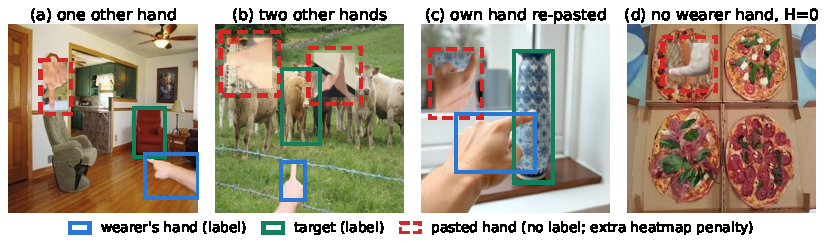
\includegraphics[width=\linewidth]{figures/ownership_examples}
  \caption{Distractor-hand pasting, produced by the training code. Pasted hands (red, dashed) come from other images (a, b) or from the same image (c), are rotated so that they rarely enter from the bottom edge, and are never labelled. A no-hand image with a pasted hand keeps the label \emph{no hand} (d).}
  \Description{Four training images. In the first two, one or two hands cut from other photos are pasted into the upper part of the image, rotated, and marked with red dashed boxes, while the wearer's pointing hand and the target keep their blue and green label boxes. In the third, a rotated copy of the wearer's own hand is pasted in the upper left. In the fourth, a pizza photo without a wearer's hand receives a pasted hand and keeps the label no hand.}
  \label{fig:ownership}
\end{figure}

\emph{Pasting.}
\begin{itemize}
\item \emph{Frequency.} With probability 0.5 for images with a hand and 0.3 for images without one, we paste one or two hand crops taken from other training images.
\item \emph{Size.} Each crop is scaled to 0.45--1.0 of its source size.
\item \emph{Orientation.} With probability 0.7, the crop is rotated by 90, 180 or 270$^\circ$ and possibly mirrored. Unlike the wearer's arm, it therefore rarely enters from the bottom edge.
\item \emph{Placement.} The crop is centred in the upper 65\% of the frame, with less than 15\% overlap with the wearer's hand and the target.
\item \emph{Blending.} The crop is blended with a feathered alpha mask and a small colour jitter.
\item \emph{Self-paste.} In 30\% of cases, the pasted crop is the wearer's own hand from the same image. Appearance alone then cannot tell the two hands apart, and the model has to use position, orientation and context.
\item \emph{Decoys.} With probability 0.15, we also paste an unlabelled patch that contains no hand, so that a pasted rectangle is not itself a cue.
\end{itemize}
Labels never change. In particular, a no-hand image with pasted hands remains \emph{no hand}, which teaches the hand gate to answer for the wearer only.

\emph{Ownership-weighted negatives.} In the hand-heatmap loss, the negative term near a pasted hand is multiplied by $1+4\,G_k$, where $G_k$ is a Gaussian ($\sigma{=}1.5$ cells) at that hand's centre. A response on another person's hand thus costs up to five times as much as one on background.

\emph{The prior this encodes.} The procedure assumes that, from a head-worn camera, the wearer's arm enters from the bottom of the frame, while other people's hands appear higher and in other orientations. This holds for most use of glasses but not always, for example when the wearer raises a hand above eye level or when a companion's hand is near the bottom of the view. Section~\ref{sec:discussion} discusses this limitation.

\subsection{Scheduled Anchor Forcing}\label{sec:forcing}
Early in training, the predicted hand centre, fingertip and target centre are close to random, so the downstream heads would read features at meaningless locations. As in scheduled sampling for sequence models~\cite{bengio2015scheduled}, we sometimes replace each anchor with its ground-truth location. This happens independently per image and per anchor, with a probability that decreases linearly from 0.5 to 0 over the first 20 epochs. From then on, training uses the model's own anchors, as at test time.

\section{Data and Evaluation Protocol}\label{sec:data}

\subsection{EgoPoint}
We train and test on the image set of EgoPoint-Ground~\cite{egopoint}, which we call EgoPoint. Its paper reports 15,338 images:
\begin{itemize}
\item 39\% (6,035) real captures with RayNeo~V3 smart glasses (12\,MP Sony IMX681 sensor);
\item 39\% (5,976) synthetically composed;
\item 22\% (3,327) LLM-generated.
\end{itemize}
These are the paper's main-text labels; its appendix calls the last two groups ``synthetic generation'' and ``image editing''. The paper describes a random 7:2:1 train:val:test split, plus a domain-adaptive split that keeps all real captures for testing. The release we use has 15,455 images split 10,837 / 1,546 / 3,072. VistaRef~\cite{li2026vistaref} and PointVG-R~\cite{li2026pointvgr} report the same counts, so our test images are theirs, minus the exclusions below. \tbd{Ask the EgoPoint-Ground authors how this release relates to the paper's splits, and state the access terms and licence.} Each positive record shows one wearer's hand pointing at one target; negatives show no hand. Per-image source labels (real, composed or generated) are \tbd{not available in our copy; if obtained, also report results on the real subset}.

\paragraph{Conversion.} We convert each record to our label format (the three flags, hand box, fingertip and target box):
\begin{itemize}
\item Negatives become 000, and their object boxes are ignored.
\item Positives with a hand box, an annotated fingertip and a target box become 111.
\item In three test records, the hand label was attached to an object and the hand was labelled as an object. We detected these by the fingertip position and swapped the labels back.
\item We dropped 232 positives: 229 without an annotated fingertip (164 train, 22 validation, 43 test) and 3 without a hand box. All 229 are flagged as unclear in the source annotations. Spot checks showed open palms, held objects, or a hand box on the hand that was not pointing.
\end{itemize}
Table~\ref{tab:data} summarises the result. Images are stored at $224\times224$; the model squashes every frame to its square $160\times160$ input, regardless of the original aspect ratio.

\begin{table}[t]
  \caption{EgoPoint after conversion. \emph{On object}: the fingertip lies inside the target box; \emph{near}: fingertip--box distance ${\leq}\,0.08$ of the image side; \emph{far}: ${>}\,0.08$.}
  \label{tab:data}
  \footnotesize
  \begin{tabular}{lrrrrrr}
    \toprule
    & & & & \multicolumn{3}{c}{Pointing at target, by distance} \\
    \cmidrule(l){5-7}
    Split & Images & No hand (000) & Pointing at target (111) & On object & Near & Far \\
    \midrule
    Train & 10,669 & 1,535 & 9,134 & 6,511 & 1,995 & 628 \\
    Validation & 1,524 & 211 & 1,313 & 922 & 297 & 94 \\
    Test & 3,029 & 425 & 2,604 & 1,796 & 599 & 209 \\
    \midrule
    Total & 15,222 & 2,171 & 13,051 & 9,229 & 2,891 & 931 \\
    \bottomrule
  \end{tabular}
\end{table}

\paragraph{Consequences for evaluation.}
\begin{itemize}
\item \emph{Test split.} Our test split has 3,029 images, 43 positives fewer than the official one. Wherever we show numbers published on the official split, we say so; those numbers are not strictly comparable (Section~\ref{sec:main}).
\item \emph{Two scenes only.} EgoPoint contains only scenes 000 and 111. The pointing and target gates therefore never see a negative example, and we report neither their accuracy nor four-class scene accuracy.
\item \emph{Distance skew.} About 70\% of targets are touched by the fingertip, and only 7\% are far. Pooled results are dominated by touched targets, so we report every target metric by distance as well. The median distance from the fingertip to the target centre is 0.12, 0.17 and 0.32 of the image side for on-object, near and far targets (test split).
\end{itemize}

\subsection{Metrics}\label{sec:metrics}
\begin{itemize}
\item \emph{Target and hand localisation.} We use the two standard grounding metrics~\cite{egopoint,li2026vistaref,li2026pointvgr}. \emph{mIoU} is the IoU between predicted and labelled box, averaged over images, with a 95\% bootstrap confidence interval (1,000 resamples~\cite{efron1994introduction}). \emph{P@$\tau$} (Precision@$\tau$) is the share of images with IoU${\geq}\tau$, for $\tau$ = 0.3, 0.5 and 0.7. Both are given in \%. Target metrics are given overall and by distance.
\item \emph{Fingertip and direction.} Fingertip error is in pixels at the $160\times160$ input (1\,px = 0.63\% of the image side). Direction error is the angle between $\hat{\dir}$ and $\dir^\star$.
\item \emph{Hand presence.} For the hand gate, we report accuracy, missed hands, false alarms and AUROC, and the two-scene accuracy (no hand versus pointing at target), with Wilson intervals~\cite{wilson1927probable} for proportions.
\item \emph{No skipped images.} Localisation is scored on every image whose label contains the part, whatever scene the model predicted, so hard images cannot be skipped.
\end{itemize}

\paragraph{Ownership test.} To test robustness to other people's hands, we paste one or two hands into every test image. The hands come from other test images, 30\% are re-pasted copies of the wearer's own hand, and their positions are fixed by a seed. Labels stay unchanged. We report:
\begin{itemize}
\item \emph{ownership accuracy}: the share of hand images in which the predicted hand centre is nearer the wearer's hand than any pasted hand;
\item how often the predicted centre falls inside a pasted hand;
\item the share of no-hand images that stay \emph{no hand}.
\end{itemize}
These distractors follow the training distribution, so this test measures robustness to that synthetic distribution and may overstate robustness in real scenes. Section~\ref{sec:own} therefore adds real frames.

\paragraph{Model selection.} The reported checkpoint has the lowest validation loss. It was fixed before we looked at the test split, and the test split was evaluated once. \tbd{Confirm: loss weights and all hyper-parameters were set on the validation split only.}

\section{Implementation and On-Glasses Deployment}\label{sec:impl}

\subsection{Training}
\paragraph{Optimisation.}
\begin{itemize}
\item AdamW~\cite{loshchilov2019decoupled}, weight decay $10^{-4}$, batch size 32.
\item One-cycle schedule~\cite{smith2019super}: peak learning rate $3\times10^{-3}$ for the heads and $3\times10^{-4}$ for the backbone, 10\% warm-up, then cosine decay.
\item Up to 180 epochs, stopping early after 25 epochs without a lower validation loss.
\item Gradient clipping at 1.0, mixed precision, seed 42.
\end{itemize}
Training took 1\,h\,40\,min on one NVIDIA Tesla T4 (47\,s per epoch). Early stopping ended it after 125 epochs; the reported checkpoint is from epoch 100. Early stopping (patience 25 on the validation loss) ended the 180-epoch one-cycle schedule before it completed. Every run in this paper uses the same rule, so all comparisons are like for like; a completed schedule would, if anything, raise the absolute numbers.

\paragraph{Augmentation.} Besides the distractor pasting of Section~\ref{sec:ownership}:
\begin{itemize}
\item horizontal flip (no vertical flip, because a wearer's hand entering from the top would contradict the ownership prior);
\item shift, scale and rotation (${\pm}5\%$, ${\pm}10\%$, ${\pm}15^\circ$; probability 0.4);
\item perspective warp (0.2);
\item brightness and contrast (${\pm}20\%$; 0.5);
\item Gaussian blur (0.2);
\item mixup~\cite{zhang2018mixup} between images of the same scene, with $\lambda\sim\mathrm{Beta}(0.2,0.2)$ folded to $\geq0.5$ and the label of the dominant image.
\end{itemize}
All augmentation is on the fly; the dataset on disk is never modified. Appendix~\ref{app:aug} lists all parameters.

\paragraph{Export.} The model is exported to ONNX (opset 17, which bilinear grid sampling requires) and to FP16. The FP16 weights take 1.6\,MB.

\subsection{Deployment on Smart Glasses}\label{sec:device}
We deploy the 160\,px model on an engineering unit of a pair of smart glasses: a pre-production test device, not a retail product. Its hardware:
\begin{itemize}
\item a smart-glasses system-on-chip paired with a low-power microcontroller;
\item a single 12\,MP ultra-wide camera (105$^\circ$) in portrait orientation, with a dedicated low-power vision NPU;
\item Wi-Fi~6 and Bluetooth~5.4 to a companion phone;
\item a 160\,mAh battery, in a frame weighing under 45\,g.
\end{itemize}
Because it is an engineering device, its power management is not tuned for production, so absolute battery figures are pessimistic. We therefore compare power between operating modes on the same unit, rather than reporting battery life. We treat the unit as a measurement platform: its pre-production software stack is not public, so we report end-to-end device measurements rather than runtime-specific details.

\paragraph{Operating modes.} We compare two ways of running pointing localisation:
\begin{itemize}
\item \emph{On the glasses:} SpatialNet runs continuously on frames from the glasses' camera.
\item \emph{Offloading:} the glasses only capture frames and transmit them to the companion phone at 0.5 frames per second, the alternative in which localisation would run on the phone or in the cloud.
\end{itemize}

\paragraph{Measurement.}
\begin{itemize}
\item the inference latency per frame;
\item the peak additional RAM used during inference, measured over the idle application with the model already loaded (the 1.6\,MB of FP16 weights are stored separately);
\item the battery drain over one minute, in each operating mode, starting from the same charge level.
\end{itemize}

The camera delivers portrait frames, whereas most EgoPoint images are landscape. The model squashes both to a square, so the deployed input has a different aspect ratio from most training images. Real-frame behaviour is assessed in Section~\ref{sec:own}.

\section{Results}\label{sec:results}

We answer five questions:
\begin{enumerate}
\item How well does SpatialNet find the pointed-at object, compared with published results of state-of-the-art and zero-shot models and with simple references (Section~\ref{sec:main})?
\item Where does it fail, by distance and by head (Section~\ref{sec:heads-results})?
\item Which design choices matter (Section~\ref{sec:ablations})?
\item Does it follow the wearer's hand when other hands are visible (Section~\ref{sec:own})?
\item How fast does it run on the glasses (Section~\ref{sec:ondevice})?
\end{enumerate}
SpatialNet numbers are from one training run (seed 42) on the 3,029 test images. \tbd{After T4, report mean $\pm$ std over three seeds.}

\subsection{Pointed-Target Localisation}\label{sec:main}

\paragraph{References.} We compare SpatialNet with two kinds of reference.
\begin{itemize}
\item \emph{Published results.} We copy these numbers and do not re-run the models.
  \begin{itemize}
  \item VistaRef~\cite{li2026vistaref} and PointVG-R~\cite{li2026pointvgr} report results on the same 3,072-image test split; ours omits 43 unclear images and the 425 images without a target. PointVG-R also reports zero-shot and fine-tuned multimodal LLMs on that split.
  \item EgoPoint-Ground's pointing-only (POG) results~\cite{egopoint} come from a different setting: zero-shot models receive the ground-truth hand box, and the evaluated subset is not stated.
  \end{itemize}
\item \emph{Simple references.} These test whether knowing where the fingertip is would be enough:
  \begin{itemize}
  \item the mean training target box at a fixed position;
  \item a box of mean training size centred on SpatialNet's predicted fingertip;
  \item the same box centred on the ground-truth fingertip.
  \end{itemize}
\end{itemize}

\begin{table}[t]
  \caption{Localisation of the pointed-at target on the EgoPoint test split. All columns compare a predicted \emph{target} box with the labelled target box; hand accuracy is in Table~\ref{tab:heads}. Our rows use the 2,604 test images with a target; the 425 no-hand images have none. mIoU and P@$\tau$ (Section~\ref{sec:metrics}) in \%, the published values multiplied by 100. We count IoU${\geq}\tau$, as does VistaRef; EgoPoint-Ground and PointVG-R count IoU${>}\tau$. \emph{Far}: P@0.5 on the 209 far targets. Latency per image on the hardware named in the text; only SpatialNet runs on the glasses.\\
  $^\ast$\,VistaRef~\cite{li2026vistaref}, Table~1, setting ``Train-Real Data Test'', BEiT-3-L backbone (226M parameters with BEiT-3-Base); test set of 3,072 images, which includes no-hand images.\\
  $^\ddagger$\,PointVG-R~\cite{li2026pointvgr}, Table~1, EgoPoint-CoT test set, built on the same 15,455-image release and 3,072-image test split.\\
  $^\dagger$\,EgoPoint-Ground~\cite{egopoint}, Table~4, pointing-only (POG) task: inference only, given the ground-truth hand box; the evaluated data subset is not stated.\\
  How the published works score images without a target is not stated; our rows exclude them.}
  \label{tab:main}
  \footnotesize
  \setlength{\tabcolsep}{4pt}
  \begin{tabular}{lrrrrrrr}
    \toprule
    Method & Params & P@0.3 & P@0.5 & P@0.7 & mIoU & Far & Latency \\
    \midrule
    \multicolumn{8}{l}{\emph{Published, trained on EgoPoint (not re-run)}} \\
    \quad VistaRef$^\ast$, image + fixed prompt & $>$226M & 97.0 & 93.9 & 82.6 & 82.0 & -- & -- \\
    \quad PointVG-R$^\ddagger$, image + instruction, SFT + RL & 7B & 88.1 & 83.6 & 74.5 & 75.7 & -- & -- \\
    \quad Qwen2.5-VL-7B$^\ddagger$, image + instruction, SFT & 7B & 68.7 & 63.6 & 56.7 & 59.8 & -- & -- \\
    \multicolumn{8}{l}{\emph{Published, zero-shot (not re-run)}} \\
    \quad Qwen2.5-VL-7B$^\ddagger$, image + instruction & 7B & 54.2 & 49.8 & 42.9 & 45.5 & -- & -- \\
    \quad Qwen3-VL-8B$^\ddagger$, image + instruction & 8B & 48.1 & 44.5 & 39.0 & 43.0 & -- & -- \\
    \quad SV-CoT$^\dagger$, image + hand box & $>$1B & 69.4 & 63.9 & 55.6 & -- & -- & -- \\
    \quad Qwen3-VL-4B$^\dagger$, image + hand box & 4B & 67.1 & 61.2 & 53.2 & -- & -- & -- \\
    \multicolumn{8}{l}{\emph{Simple references}} \\
    \quad Mean training box, fixed position & 0 & 41.3 & 9.6 & 0.9 & 27.4 & 4.3 & -- \\
    \quad Mean-size box at predicted fingertip & 0.72M & 43.5 & 11.2 & 0.9 & 28.8 & 0.0 & -- \\
    \quad Mean-size box at true fingertip (oracle) & -- & 43.6 & 11.4 & 1.0 & 29.0 & 0.0 & -- \\
    \midrule
    \textbf{SpatialNet} (image only, seed 42) & 0.72M & 78.6 & 58.9 & 31.8 & 53.3 & 25.4 & \xx\,ms \\
    \quad $\pm$ std over 3 seeds & & \xx & \xx & \xx & \xx & \xx & \\
    \bottomrule
  \end{tabular}
\end{table}

\paragraph{Results.} Table~\ref{tab:main} gives three findings.
\begin{itemize}
\item \emph{The target head does real work.} Knowing the fingertip is not enough: a mean-size box at the true fingertip reaches a P@0.5 of only 11.4\% (12.0\% when shifted by the mean training offset), because target sizes vary widely (2.6\% to 44\% of the image area, 10th to 90th percentile). SpatialNet reaches 58.9\%.
\item \emph{Large models trained on EgoPoint are far more accurate.} SpatialNet is 35 points below VistaRef in P@0.5 and 51 points below in P@0.7, where its boxes are least precise; in mIoU the gap is 29 points (53.3 against 82.0). It is 25 points below PointVG-R, and 4.7 points below Qwen2.5-VL-7B fine-tuned on the same data.
\item \emph{It is comparable to zero-shot multimodal LLMs.}
  \begin{itemize}
  \item SpatialNet's P@0.5 (58.9\%) and mIoU (53.3\%) are above the zero-shot Qwen2.5-VL-7B (49.8\%, 45.5\%) and Qwen3-VL-8B (44.5\%, 43.0\%) reported by PointVG-R.
  \item Those numbers average over all 3,072 test images, including 425 without a target. If those were scored as failures, Qwen2.5-VL-7B would reach about 57.8\% P@0.5 and 52.8\% mIoU on the images with a target, on a par with SpatialNet.
  \item The zero-shot models draw tighter boxes: their P@0.7 (39.0--42.9\%) exceeds SpatialNet's (31.8\%).
  \item SpatialNet finds the right region far more often: P@0.3 of 78.6\% against 48.1--54.2\%.
  \item Against zero-shot models that are given the true hand box, it is slightly lower in P@0.5 (61.2--63.9\%).
  \end{itemize}
  We therefore claim parity at a fraction of the size, not superiority.
\item \emph{These comparisons are indicative only.} The published rows count IoU${>}\tau$, include no-hand test images scored in a way the papers do not state, and in one case use an unstated subset.
\item \emph{Cost.} VistaRef reports 22.9 images/s on a GPU, and the multimodal LLMs need billions of parameters. SpatialNet runs on the glasses in \xx\,ms \tbd{T2}.
\end{itemize}

\subsection{Per-Head Accuracy and Target Distance}\label{sec:heads-results}

Table~\ref{tab:heads} breaks the result down by head and by fingertip--target distance, and Figure~\ref{fig:curves} shows the IoU success curves.

\begin{table}[t]
  \caption{Accuracy of each head by fingertip--target distance (test split, pointing-at-target images). Fingertip error in pixels at the $160\times160$ input; direction error in degrees. mIoU and P@0.5 in \%; brackets: 95\% bootstrap confidence intervals of the mIoU.}
  \label{tab:heads}
  \footnotesize
  \setlength{\tabcolsep}{4pt}
  \begin{tabular}{lrrrrrrrr}
    \toprule
    & \multicolumn{2}{c}{Hand} & \multicolumn{2}{c}{Fingertip (px)} & \multicolumn{2}{c}{Direction ($^\circ$)} & \multicolumn{2}{c}{Target} \\
    \cmidrule(lr){2-3}\cmidrule(lr){4-5}\cmidrule(lr){6-7}\cmidrule(l){8-9}
    Distance (images) & mIoU & P@0.5 & mean & ${<}5$\,px & mean & ${<}15^\circ$ & mIoU [CI] & P@0.5 \\
    \midrule
    On object (1,796) & 73.7 & 92.3 & 3.79 & 84.4 & 36.0 & 39.7 & 57.9 [56.8, 59.0] & 66.0 \\
    Near (599) & 73.7 & 93.5 & 4.09 & 78.8 & 22.0 & 54.9 & 47.8 [45.8, 49.8] & 49.2 \\
    Far (209) & 72.7 & 92.8 & 4.16 & 80.9 & 29.0 & 36.8 & 29.8 [26.0, 33.6] & 25.4 \\
    \midrule
    All (2,604) & 73.7 & 92.6 & 3.89 & 82.8 & 32.2 & 43.0 & 53.3 [52.3, 54.3] & 58.9 \\
    \bottomrule
  \end{tabular}
\end{table}

\begin{figure}[t]
  \centering
  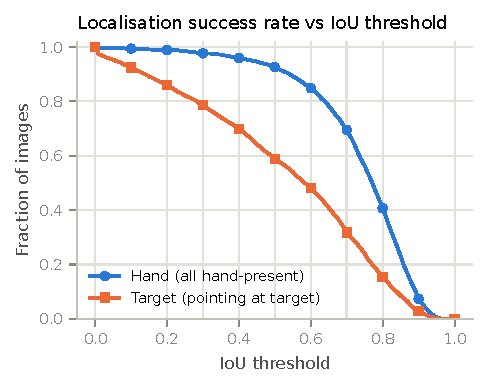
\includegraphics[width=0.48\linewidth]{figures/results/iou_success_rate}\hfill
  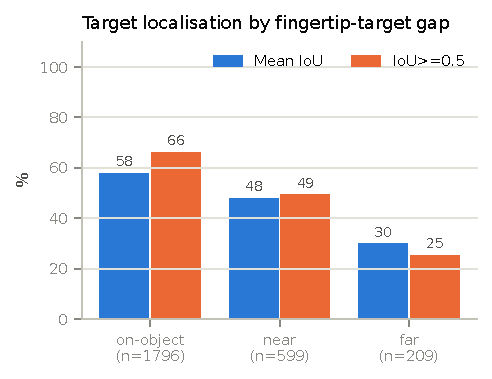
\includegraphics[width=0.48\linewidth]{figures/results/target_iou_by_gap}
  \caption{Left: share of test images whose hand or target box reaches each IoU threshold. Right: target mIoU and P@0.5 for touched, near and far targets.}
  \Description{Left: two curves of success rate against IoU threshold; the hand curve stays above 0.9 up to IoU 0.5 and falls after 0.7, while the target curve falls steadily, reaching 0.59 at IoU 0.5 and 0.32 at 0.7. Right: bars of mean target IoU and IoU above 0.5: 58 and 66 percent for touched targets, 48 and 49 for near targets, 30 and 25 for far targets.}
  \label{fig:curves}
\end{figure}

\paragraph{Hand presence.} The hand gate separates no-hand from pointing frames with 98.6\% accuracy (95\% CI 98.1--98.9) and AUROC 0.998. It misses 15 of 2,604 hands (0.6\%) and raises false alarms on 28 of 425 no-hand frames (6.6\%). Choosing the threshold on validation so that no hand is missed (0.22) removes the misses but raises false alarms to 117 (27.5\%), so we keep 0.5.

\paragraph{Where the errors come from.}
\begin{itemize}
\item \emph{Hand and fingertip are not the bottleneck.} The hand box and fingertip are equally good for all distances (hand P@0.5 of 92--94\%; about 4\,px fingertip error, 2.5\% of the image side).
\item \emph{The target falls off with distance.} Target P@0.5 drops from 66.0\% for touched targets to 49.2\% near and 25.4\% far (mIoU from 57.9 to 47.8 and 29.8).
\item \emph{The direction is coarse.} Its median error is 18.6$^\circ$, and only 36.8\% of far targets have an error below 15$^\circ$. At a median fingertip--target distance of 0.32 image widths, 15$^\circ$ already moves the ray by about 0.08 image widths, the size of a small object. The error is largest for touched targets (36$^\circ$), where the direction to the target centre is ill-defined and matters least.
\item \emph{Size is regressed towards the mean.} The predicted target centre lies inside the labelled box in 84.8\% of images. Giving the model the true size with its own centre would raise P@0.5 to 70.4\%; giving it the true centre with its own size would raise it to 72.3\%. Errors in position and in extent therefore contribute about equally. Small targets (under 3\% of the image) are predicted about 1.9 times too large, and reach a P@0.5 of only 36.9\%.
\end{itemize}

\subsection{Ablations}\label{sec:ablations}

We retrain the model without one component at a time, with the seed and settings of the main run:
\begin{itemize}
\item \textbf{A1} no distractor pasting and no ownership weighting;
\item \textbf{A2} no geometric consistency terms ($\mathcal{L}_{\mathrm{ray}}$ and the hand-axis term);
\item \textbf{A3} no ray conditioning of the target head (no $G^t$; 13,105 fewer parameters).
\end{itemize}
\tbd{A4 (recommended now that efficiency is the main claim): no instance-anchored chain, so the heads read the globally pooled vector (\texttt{--no\_anchor\_chain}). This is the same-size plain baseline; it shows whether the design, and not just the small backbone, explains the accuracy.}
Each ablation was trained once. Instead of seed variation, we report a paired bootstrap over test images: we resample the 2,604 images and recompute the difference between the full model and the ablation on the same images, which yields a 95\% confidence interval for each difference.

\begin{table}[t]
  \caption{Ablations (one seed each). Differences from the full model with 95\% paired-bootstrap intervals; intervals that exclude 0 are in bold. Ownership: ownership accuracy on the synthetic multi-hand test.}
  \label{tab:ablation}
  \footnotesize
  \setlength{\tabcolsep}{4pt}
  \begin{tabular}{lrrrrrr}
    \toprule
    Variant & Target mIoU & P@0.5 & Far P@0.5 & Hand mIoU & Tip (px) & Ownership \\
    \midrule
    Full model (seed 42) & 53.3 & 58.9 & 25.4 & 73.7 & 3.89 & 99.7 \\
    A1 no distractors / ownership weight & \xx & \xx & \xx & \xx & \xx & \xx \\
    A2 no geometric consistency terms & \xx & \xx & \xx & \xx & \xx & \xx \\
    A3 no ray conditioning & \xx & \xx & \xx & \xx & \xx & \xx \\
    \bottomrule
  \end{tabular}
\end{table}

\paragraph{Results.} \tbd{Write one claim per row, only as strong as its interval:}
\begin{itemize}
\item \tbd{A3 tests contribution C1. Far targets reach only 25.4\% with the ray conditioning; if A3 is not significantly lower, the ray prior does not help and C1 must be weakened in the abstract and introduction.}
\item \tbd{A2 tests whether the two consistency terms help, mostly on far targets.}
\item \tbd{A1 should mainly affect ownership; report any cost on clean-image accuracy. See the caveat in Section~\ref{sec:own}.}
\end{itemize}
The loss weights were not searched (Appendix~\ref{app:weights}): A2 covers the two non-standard terms, and the remaining eleven are standard box, keypoint, heatmap and focal losses.

\subsection{Following the Wearer's Hand}\label{sec:own}

\paragraph{Synthetic distractors.} With one or two pasted hands in each test image, the model's hand still lies nearer the wearer's hand than any pasted hand in 99.7\% of hand images (Table~\ref{tab:own}), and other metrics barely change. This is weaker evidence than it looks:
\begin{itemize}
\item The pasted hands follow the training distribution.
\item The ownership metric is easy under that distribution. In the first training epoch, when the hand IoU was only 0.38, ownership accuracy on training batches was already 93\%, because pasted hands sit in the upper part of the frame and the wearer's hand in the lower part.
\end{itemize}
The more informative number is that pasted hands rarely turn a no-hand frame into a hand frame: 91.8\% of no-hand frames stay \emph{no hand}, against 93.4\% without pasted hands. Whether the training recipe is needed at all is answered by A1, and robustness to real bystanders by the real-frame check below.

\paragraph{Real frames.} \tbd{Fill in when T5 is done:}
\begin{itemize}
\item We recorded \tbd{N} clips with the glasses in which another person's hand is visible, sometimes pointing, with \tbd{consent procedure}, and sampled \tbd{100--150} frames.
\item Two annotators independently labelled the predicted hand in each frame as the wearer's, another person's, or missed.
\item We report ownership accuracy with a Wilson interval and inter-annotator agreement (Cohen's $\kappa$).
\end{itemize}
Figure~\ref{fig:own-real} shows examples.

\begin{table}[t]
  \caption{Ownership on test images with one or two pasted hands (synthetic), and on real frames with other people's hands (T5). All values in \%. \emph{On other hand}: predicted hand centre inside a pasted hand. \emph{No hand kept}: no-hand images still classed as no hand.}
  \label{tab:own}
  \footnotesize
  \begin{tabular}{lrrrr}
    \toprule
    & Ownership accuracy & On other hand & No hand kept & Target P@0.5 \\
    \midrule
    Full model, clean test images & -- & -- & 93.4 & 58.9 \\
    Full model, pasted hands & 99.7 [99.4, 99.9] & 0.2 & 91.8 & 60.1 \\
    A1, pasted hands & \xx & \xx & \xx & \xx \\
    \midrule
    Full model, real frames (\tbd{N}) & \xx\ [\xx, \xx] & \xx & -- & -- \\
    \bottomrule
  \end{tabular}
\end{table}

\begin{figure}[t]
  \centering
  \phfig{\linewidth}{3.2cm}{Six real frames from the glasses with another person's hand in view: predicted wearer's hand, fingertip, ray and target (T5). Include at least one failure.}
  \caption{Real frames with other people's hands. \tbd{Insert after T5.}}
  \Description{To be inserted: six photos from the glasses showing SpatialNet's outputs while another person's hand is visible.}
  \label{fig:own-real}
\end{figure}

\subsection{On-Device Performance}\label{sec:ondevice}

Table~\ref{tab:device} reports cost on the evaluation machine and on the glasses.

\begin{table}[t]
  \caption{Inference cost at batch size 1 and $160\times160$ input. Server numbers use PyTorch eager mode on the 4-core Kaggle virtual machine used for evaluation and are given for reference only; at this model size, they are dominated by framework overhead.}
  \label{tab:device}
  \footnotesize
  \begin{tabular}{llrr}
    \toprule
    Platform and measure & Runtime / precision & Median & p90 \\
    \midrule
    Server CPU, 1 thread & PyTorch FP32 & 25.7\,ms & 28.0\,ms \\
    Server CPU, 4 threads & PyTorch FP32 & 25.8\,ms & 27.0\,ms \\
    Server GPU, NVIDIA Tesla T4 & PyTorch FP32 & 15.9\,ms & 16.3\,ms \\
    \midrule
    Glasses, model only & \tbd{runtime, unit, precision} & \xx\,ms & \xx\,ms \\
    Glasses, camera frame to result & \tbd{same} & \xx\,ms & \xx\,ms \\
    Glasses, sustained throughput (60\,s) & & \multicolumn{2}{r}{\xx\ frames/s} \\
    Glasses, peak memory / battery per 10\,min & & \multicolumn{2}{r}{\xx\,MB / \xx\%} \\
    Glasses vs.\ PyTorch, 100 test images & & \multicolumn{2}{r}{\xx\% same scene; box IoU \xx} \\
    \bottomrule
  \end{tabular}
\end{table}

\paragraph{Results.} Running the FP16 weights in half precision gives the same target IoU as FP32 on 320 validation images (0.510 in both), so halving the model size costs no accuracy. \tbd{T2: model latency against the camera's frame interval, end-to-end latency against a 100--200\,ms interactive budget, and the cost gap to the GPU-based models of Table~\ref{tab:main} (VistaRef: 22.9 images/s on a GPU). If capture or conversion dominates the end-to-end time rather than the model, say so.}

\subsection{Qualitative Results and Failure Analysis}\label{sec:qual}

Figure~\ref{fig:qual} shows typical successes and failures. We sorted the 558 test images with target IoU $<$ 0.3 (21.4\%) by rule:
\begin{itemize}
\item \emph{Right object, wrong extent} (36\%): the predicted centre lies inside the labelled box. These are mostly touched targets (137 of 199), for example part of a bed instead of the whole bed.
\item \emph{Wrong direction} (33\%): direction error over 45$^\circ$.
\item \emph{Wrong object despite a reasonable direction} (31\%): mostly near and far targets (130 of 171), typically a similar object next to the labelled one along the ray.
\item \emph{Hand missed} (1\%).
\end{itemize}
Some labelled targets are ambiguous: in the ``wrong direction'' example, the finger touches the bowl but the label is an apple above it. \tbd{Inspect a random sample of 50 failures and report the share with a questionable label.}

\begin{figure}[t]
  \centering
  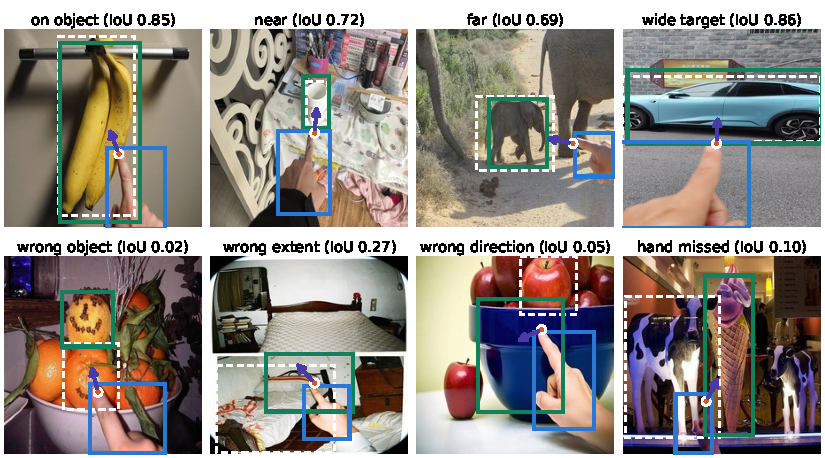
\includegraphics[width=\linewidth]{figures/qualitative}
  \caption{Successes (top) and failures (bottom) on EgoPoint test images: predicted hand (blue), fingertip and direction, and target (green); labelled target dashed. Bottom row, one example per failure type of Section~\ref{sec:qual}.}
  \Description{Eight egocentric images. Top row: correct target boxes for bananas touched by the finger, a cup near the finger, a young elephant far from the finger, and a car. Bottom row: a box on the wrong orange in a bowl of oranges, a box on part of a bed instead of the labelled bed, a box on a bowl while the label is an apple above it, and a frame where the hand gate missed the hand.}
  \label{fig:qual}
\end{figure}

\section{Discussion}\label{sec:discussion}

\paragraph{What a single-image, single-pass CNN can and cannot do.} The results separate the task into two parts.
\begin{itemize}
\item \emph{Easy at this size.} Finding the wearer's hand, the fingertip and whether a hand is present works well: 92.6\% hand IoU${\geq}0.5$, 3.9\,px fingertip error, and AUROC 0.998.
\item \emph{Hard at this size.} Deciding which object the finger refers to, and how far that object extends, is what the large models do much better. Our errors split about evenly between wrong extent, wrong direction and wrong object (Section~\ref{sec:qual}).
\end{itemize}
A 0.72M CNN at $160\times160$ therefore makes a good always-on front end: it can trigger and crop for a heavier model, but should not be expected to reach large-model accuracy alone.

\paragraph{What the design contributes.} \tbd{Rewrite once Table~\ref{tab:ablation} is filled in, keeping only the statements its intervals support; add A4 (no anchor chain) as the same-size plain baseline.} The design rests on two choices, both cheap (13K parameters each):
\begin{itemize}
\item \emph{Anchoring.} Every head reads features where the previous head looked, so the chain stays on one hand instance.
\item \emph{Learned, safe geometry.} The ray enters as a zero-initialised log-prior. It cannot hurt at the start of training and is used only as far as it helps.
\end{itemize}
Wearer-awareness from distractor pasting is a third, secondary choice. Its evidence is so far synthetic (Section~\ref{sec:own}).

\paragraph{Deployment caveat.} The heads use bilinear sampling (\texttt{grid\_sample}, ONNX opset 16 or later), which not every mobile NPU runtime supports. \tbd{T2: state whether it ran on the NPU or fell back to the CPU.}

\paragraph{Why most targets are touched, and what that implies.} Where people point at distant objects depends on the eye as well as the arm: modelling the dominant eye makes pointing rays markedly more accurate~\cite{plaumann2018towards}, and common ray-casting models show systematic offsets~\cite{mayer2015modeling}. If wearers align the fingertip with the target from the eye, a camera next to the eye sees the target at or just behind the fingertip. This is consistent with about 70\% of EgoPoint targets containing the fingertip in the image, although part of EgoPoint is staged or generated \tbd{confirm}. It has two consequences:
\begin{itemize}
\item For such targets, the fingertip tells \emph{where} the object is but not \emph{how large} it is: a mean-size box at the true fingertip reaches IoU${\geq}0.5$ in only 11.4\% of test images (Table~\ref{tab:main}). On touched objects, the target head mainly has to estimate the object's extent.
\item The ray matters for the remaining near and far targets, where the finger points away from the line of sight. This subset is small (7\% far), so it needs its own metrics rather than pooled averages.
\end{itemize}

\paragraph{Limitations.}
\begin{itemize}
\item \emph{Two scenes.} The pointing and target gates were never trained or tested against negatives (Section~\ref{sec:data}). In deployment, a non-pointing hand may therefore be read as pointing, and the cascade's middle states are untested. A dataset with non-pointing hands and pointing without a target is needed before relying on them.
\item \emph{Ownership.} Our distractors are synthetic and encode the prior that the wearer's arm enters from the bottom of the view. The real-frame check (Section~\ref{sec:own}) is small. A wearer pointing upward from a raised arm, or a companion's hand close to the wearer's, can break the prior.
\item \emph{Target extent from a local window.} The target size is regressed from a $3\times3$ neighbourhood of the stride-8 map around the predicted centre. That window cannot see the edges of large objects, and at $160\times160$ it resolves small ones poorly. This matches the observed bias: small targets come out too large, large ones too small, and IoU${\geq}0.7$ reaches only 31.8\%. Sampling the size from a larger or box-shaped region, or using a higher input resolution, are the obvious next steps.
\item \emph{A coarse direction.} The direction error (median 18.6$^\circ$) is large for far targets, where the ray matters most, and limits them to 25.4\% IoU${\geq}0.5$.
\item \emph{A 2D ray.} The ray lives in the image plane. Objects at different depths along the same image ray are told apart only by appearance, and the eye--camera offset is ignored. Depth, or a second view, could resolve such cases.
\item \emph{Single frames.} The model has no temporal context. Detecting a pointing \emph{event}, as opposed to a pointing frame, and smoothing the target over a short window are left to the application.
\item \emph{Dataset coverage.} Results come from one dataset with mostly landscape, partly synthetic images and unknown demographic coverage (for example, skin tone and handedness). Flip augmentation covers left hands only geometrically. Evaluation on real, diverse glasses footage is the most important next step.
\item \emph{Baselines.} We copied the published state-of-the-art results instead of re-running those models, and two of them use different inputs or subsets. The VLMs were used zero-shot with \tbd{one prompt}. Large grounding models are clearly more accurate. Our claim is the operating point, with accuracy reported next to its cost, not superiority.
\end{itemize}

\paragraph{Implications for glasses interfaces.} A model of this size can run continuously and act as a gate for more expensive components:
\begin{itemize}
\item \emph{Crops instead of frames.} Only when the glasses detect a pointing frame with a confident target does a recogniser or assistant run, and then on the target crop instead of the full frame. This reduces computation, bandwidth and the amount of bystander imagery that leaves the device. \tbd{Quantify if T2 measured it; otherwise keep as a design implication.}
\item \emph{Confirmation for far targets.} Because far targets are where errors concentrate (Section~\ref{sec:heads-results}), interfaces should confirm the selection, for example by naming the object or highlighting it, before acting on it.
\end{itemize}

\section{Ethics and Privacy}\label{sec:ethics}

\paragraph{Bystanders.} A head-worn camera sees people who did not consent to being recorded.
\begin{itemize}
\item SpatialNet runs on the glasses, so localisation needs no frame to leave the device.
\item A downstream step can be limited to the target crop and to moments when the wearer points.
\item SpatialNet is trained to ignore other people's hands. It does not detect, identify or track people.
\end{itemize}
On-device processing still does not remove the need for visible recording indicators; the developer unit has user- and bystander-facing LEDs \tbd{confirm whether this may be stated}.

\paragraph{Data.} EgoPoint is used under its licence \tbd{name the licence; state whether the converted labels may be shared}. The images shown in this paper come from its test and training splits. \tbd{T5 and T6: describe consent, the ethics approval or exemption (with reference number after review), data retention, and the avoidance of bystanders' faces.}

\paragraph{Availability.} \tbd{Anonymised link to the code, conversion script, trained weights and evaluation outputs.}

\section{Conclusion}\label{sec:conclusion}
SpatialNet localises the object a smart-glasses wearer points at, from a single frame, with 0.72M parameters and one forward pass. It does so by chaining instance-anchored heads (hand, fingertip, direction, target) and by conditioning the target search on ray coordinates derived from its own predictions. Training with pasted, unlabelled hands teaches it to follow the wearer's hand. \tbd{One sentence with the key T1 and T2 numbers.} The main open problems are pointing scenes that EgoPoint does not contain, real bystander hands, and far targets along ambiguous rays. We expect progress on them to come from richer egocentric pointing data at least as much as from larger models.


\bibliographystyle{ACM-Reference-Format}
\bibliography{references}

\appendix
\section{Loss Weights}\label{app:weights}

Table~\ref{tab:weights} lists the 13 loss terms and their weights. \tbd{One true sentence on how the weights were set, e.g.: set by hand during development so that the weighted terms had similar magnitudes early in training, judged on the validation split only; no search on the test split.}

\begin{table}[h]
  \caption{Loss terms, their supervision, and weights.}
  \label{tab:weights}
  \footnotesize
  \begin{tabular}{llll}
    \toprule
    Term & Loss & Supervision & Weight \\
    \midrule
    Hand box & 1 $-$ CIoU & hand box & 0.10 \\
    Fingertip & Wing ($w{=}0.5$, $\epsilon{=}0.1$) & fingertip & 0.18 \\
    Direction & 1 $-$ cosine & fingertip $\to$ target centre & 0.03 \\
    Target box & 1 $-$ SIoU & target box & 0.45 \\
    Target box, auxiliary & 1 $-$ IoU & target box & 0.10 \\
    Hand gate & focal BCE, positives $\times3$ & $H$ & 0.08 \\
    Pointing gate & focal BCE, positives $\times2$ & $P$ (hand images) & 0.10 \\
    Target gate & focal BCE, positives $\times2$ & $T$ (pointing images) & 0.06 \\
    Ray alignment & distance to ray $+$ 0.5 $\cdot$ behind & none (predictions only) & 0.08 \\
    Hand axis & hinge outside a $60^\circ$ cone & none (predictions only) & 0.02 \\
    Hand heatmap & penalty-reduced focal, ownership-weighted & hand centre & 0.10 \\
    Fingertip heatmap & penalty-reduced focal & fingertip & 0.10 \\
    Target heatmap & penalty-reduced focal & target centre & 0.10 \\
    \bottomrule
  \end{tabular}
\end{table}

\section{Augmentation Parameters}\label{app:aug}

\begin{table}[h]
  \caption{Training-time augmentation, applied on the fly; each training image is seen once per epoch as a new random variant. Validation and test images are only resized and normalised.}
  \label{tab:aug}
  \footnotesize
  \begin{tabular}{lp{0.62\linewidth}}
    \toprule
    Step & Setting \\
    \midrule
    Distractor hands & 1--2 hands with probability 0.5 (hand images) or 0.3 (no-hand images); scale 0.45--1.0; rotation by 90/180/270$^\circ$ and optional mirror with probability 0.7; centre in the top 65\% of the frame; overlap with the wearer's hand and the target below 15\%; feathered alpha (12\% of the crop size); colour jitter; 30\% self-paste; pool of 512 donor crops, half from pointing hands \\
    Decoy patch & unlabelled non-hand patch from a no-hand image, with probability 0.15 \\
    Horizontal flip & 0.5 \\
    Shift / scale / rotate & ${\pm}5\%$ / ${\pm}10\%$ / ${\pm}15^\circ$, probability 0.4 \\
    Perspective & scale 0.02--0.05, probability 0.2 \\
    Brightness / contrast & ${\pm}20\%$, probability 0.5 \\
    Gaussian blur & kernel 3--5, probability 0.2 \\
    Mixup & within the same scene, $\lambda\sim\mathrm{Beta}(0.2,0.2)$ folded to ${\geq}0.5$, label of the dominant image, every batch \\
    Anchor forcing & ground-truth anchors with probability 0.5 decaying to 0 over 20 epochs \\
    \bottomrule
  \end{tabular}
\end{table}

\section{Vision--Language Model Prompts}\label{app:vlm}

\tbd{For each model: name, version or snapshot, access date, and decoding settings (temperature, maximum tokens); the exact prompt; the expected output format and how it was parsed into a box (coordinate convention, normalisation); the share of answers that could not be parsed; and the latency measurement setup.}


\end{document}
